\section{Risultati}
\setlength{\TPboxrulesize}{0pt}
\textblockrulecolour{white}
\textblockcolour{white}
\setbeamercolor*{item}{fg=black}

\begin{frame}
\frametitle{Summer Days}
\begin{center}

{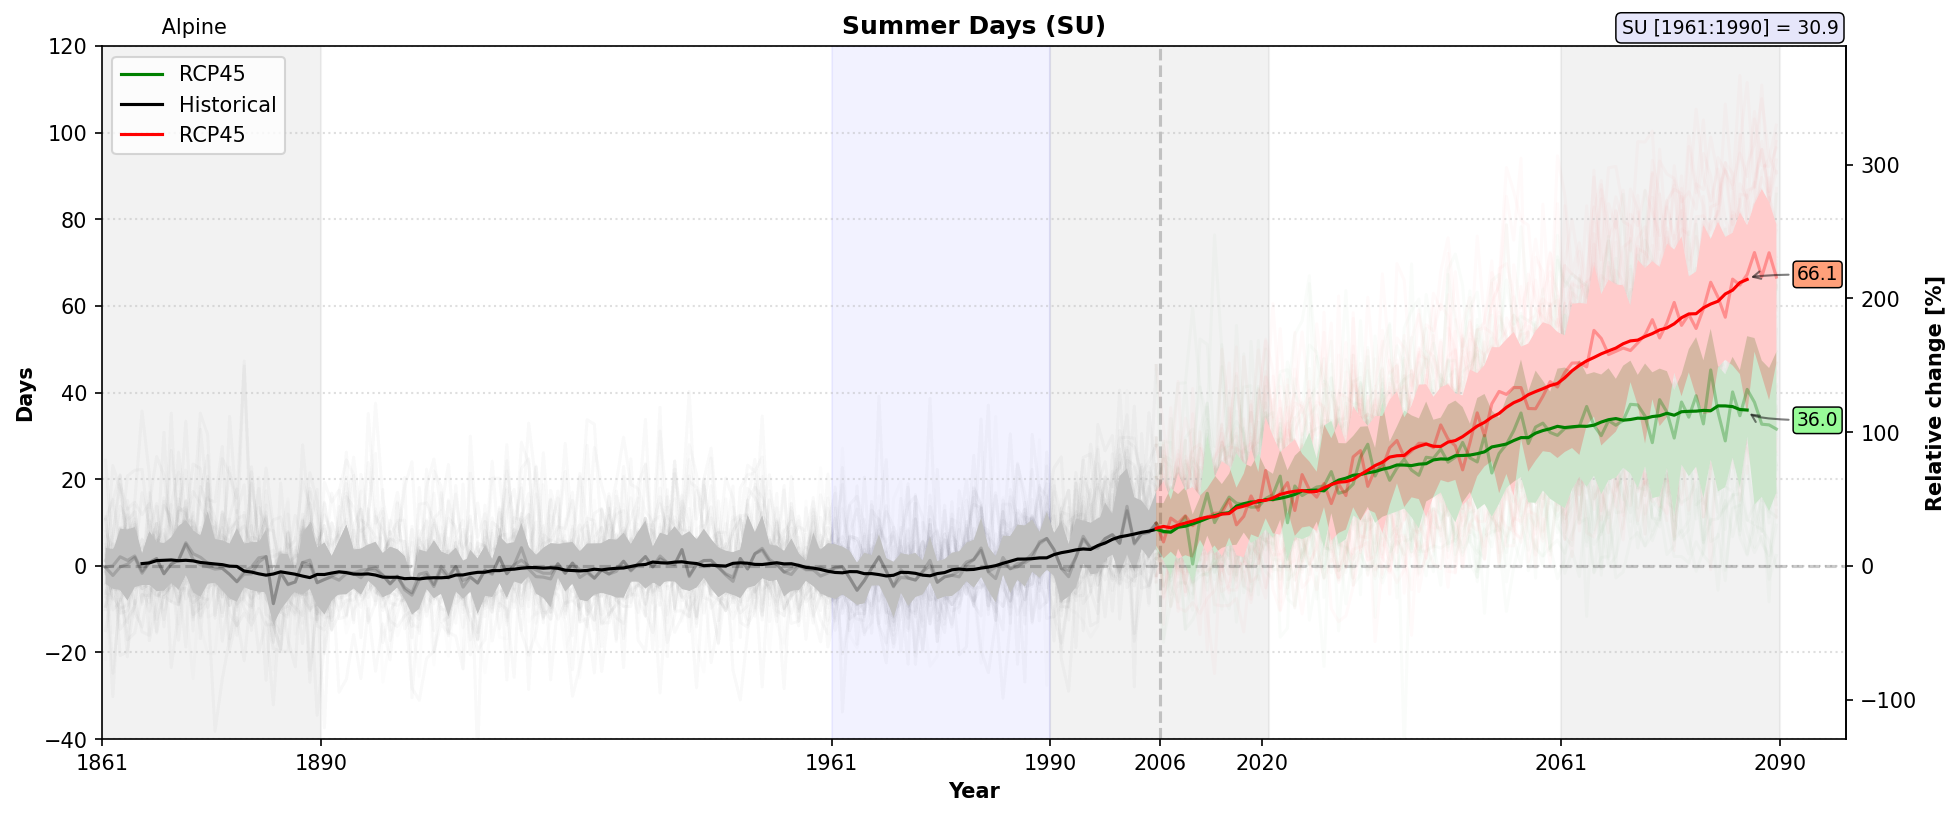
\includegraphics[width=0.8\textwidth]{risultati/su_Alpine_Models_ts_lim_120}} 
{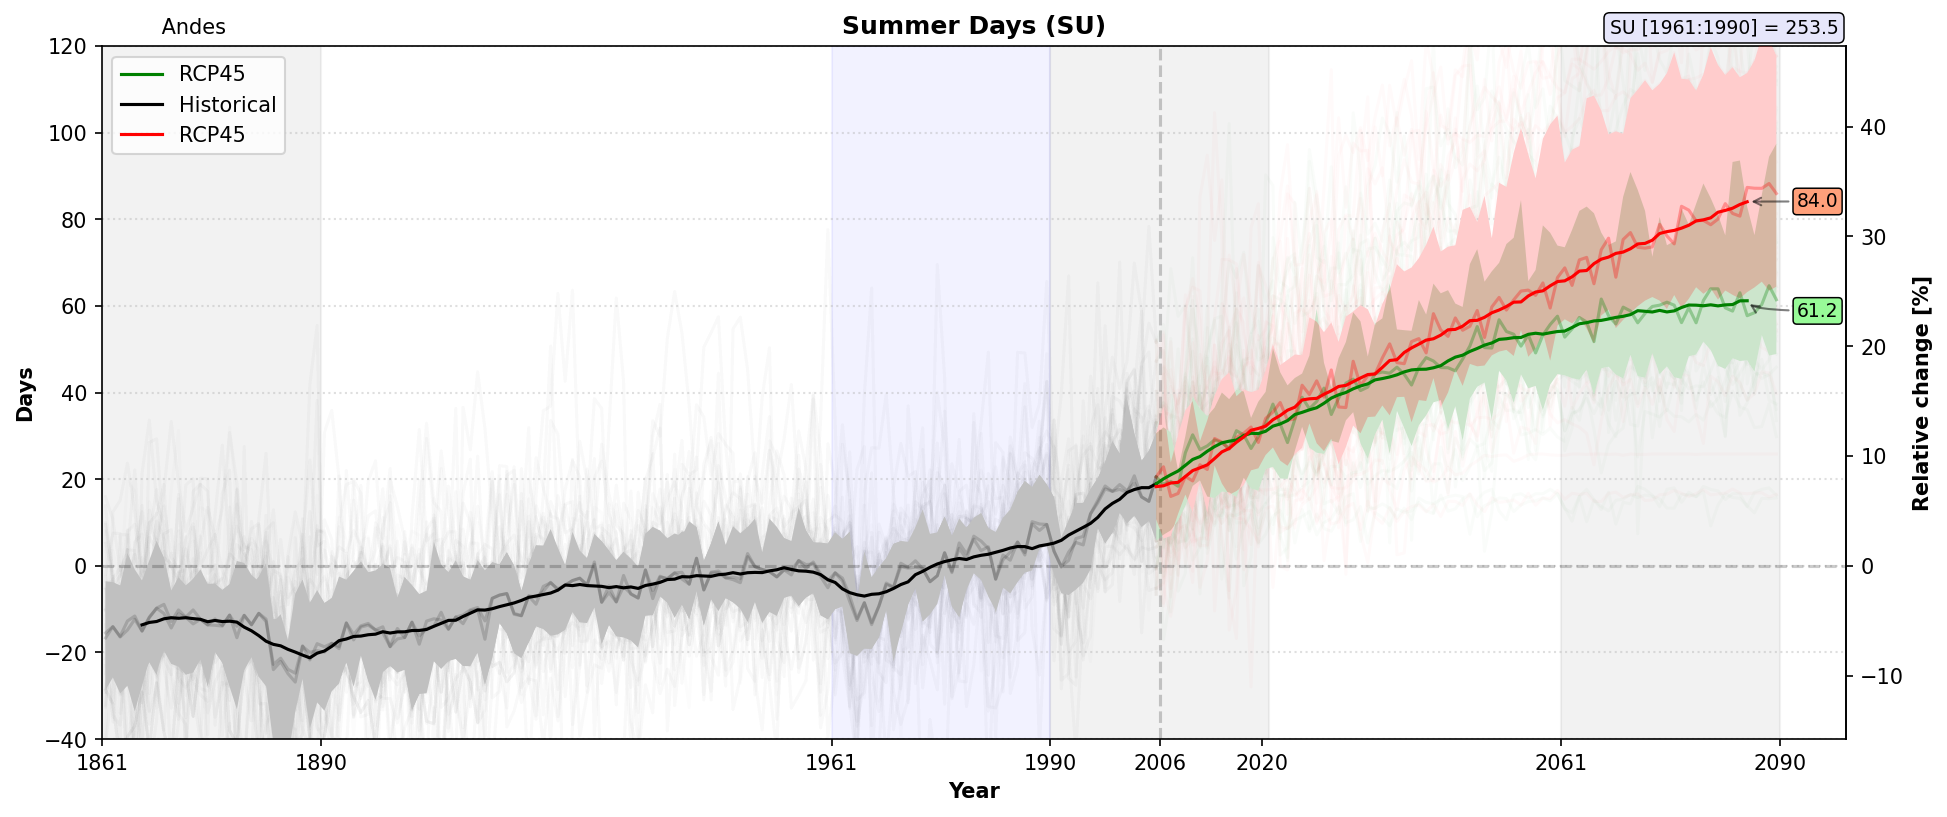
\includegraphics[width=0.8\textwidth]{risultati/su_Andes_Models_ts_lim_120}}
\end{center}

{ \scriptsize
  \begin{textblock}{1.8}(0.6,3)
     {\color{gray} Le Alpi}
  \end{textblock}
}

{ \scriptsize
  \begin{textblock}{1.8}(0.6,9.5)
     {\color{gray} Le Ande}
  \end{textblock}
}


{ \tiny
  \begin{textblock}{3}(14,3)
     {\color{CadetBlue}   \texttt{31 gg : Rif}} \\
     {\color{red}         \texttt{66 gg : 214\% }}\\
     {\color{ForestGreen} \texttt{36 gg : 116\% }}
  \end{textblock}
}

{ \tiny
  \begin{textblock}{3}(14,9.5)
     {\color{CadetBlue}   \texttt{253 gg : Rif}} \\
     {\color{red}         \texttt{ 84 gg : 33\% }} \\
     {\color{ForestGreen} \texttt{ 61 gg : 24\%  }}
  \end{textblock}
}




\end{frame}

%---------------------------------------------------
\begin{frame}
\frametitle{Summer Days}
\begin{center}

{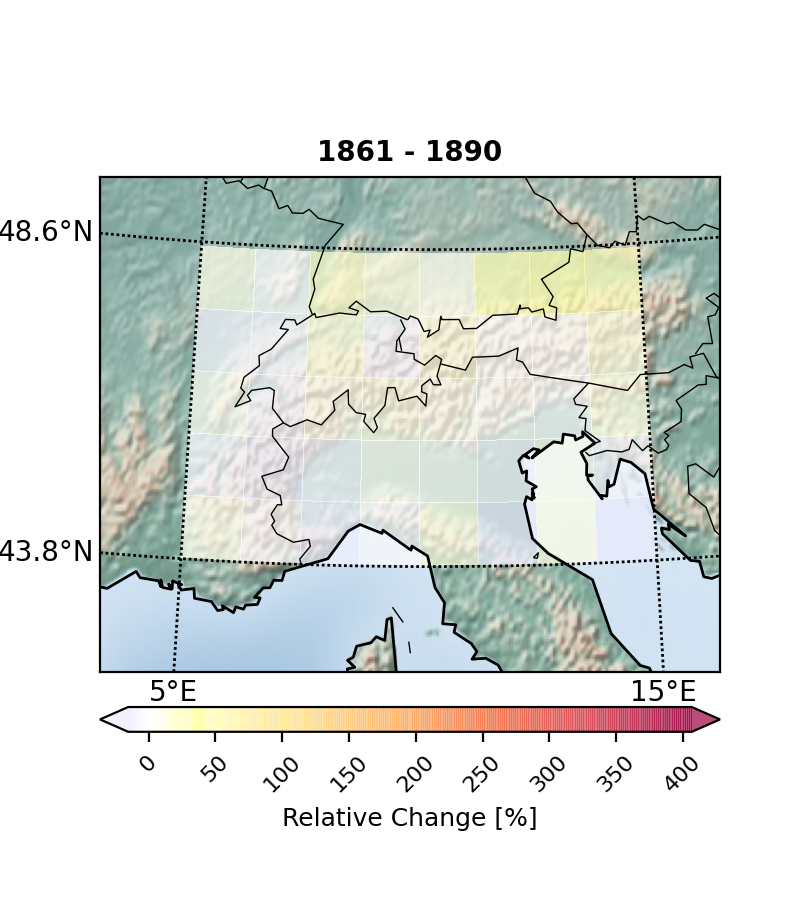
\includegraphics[trim=0 71 0 40, clip,width=.41\textwidth] {risultati/su_past_1861-1890_sub_rel}}
{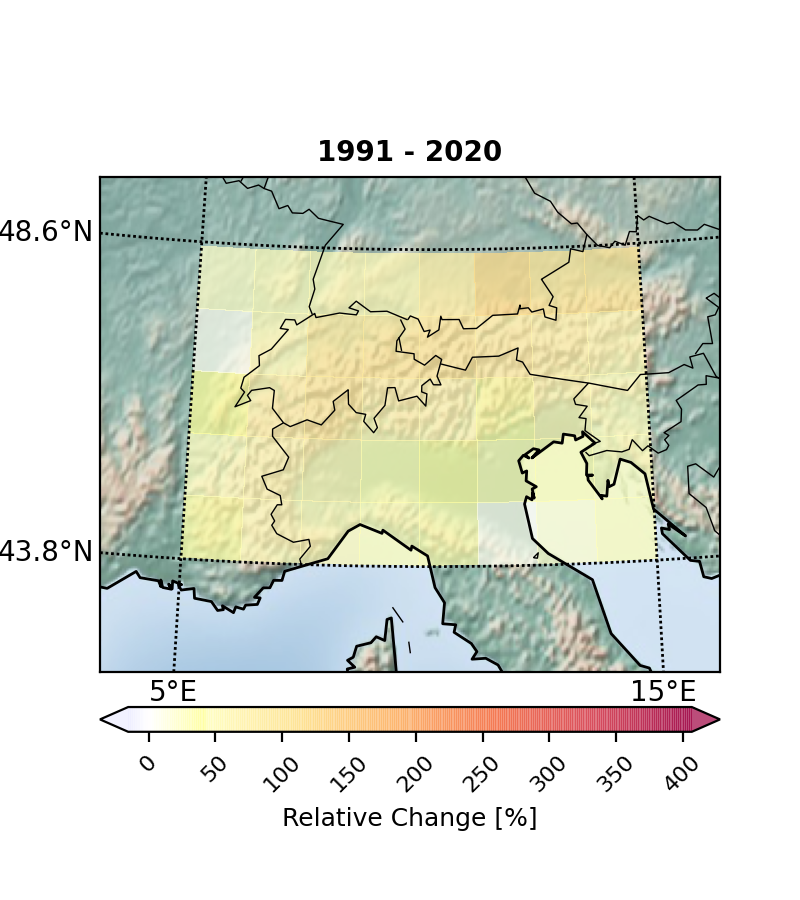
\includegraphics[trim=0 71 0 40, clip,width=.41\textwidth] {risultati/su_present_1991-2020_sub_rel}}
{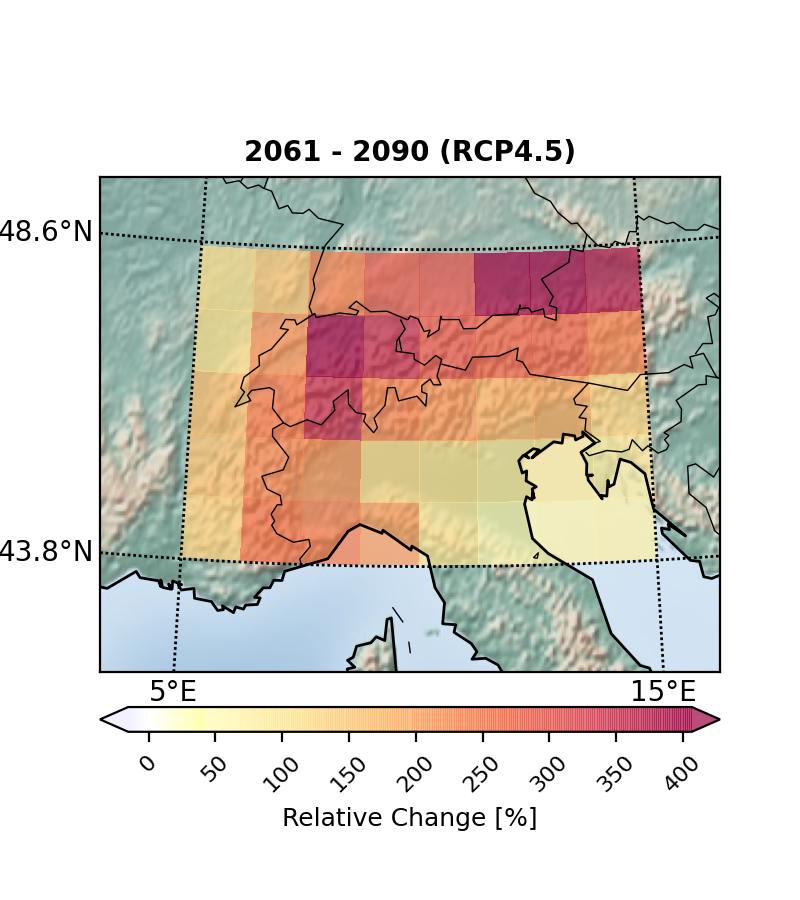
\includegraphics[trim=0 13 0 40, clip,width=.41\textwidth] {risultati/su_future_2061-2090_sub_rel45}}
{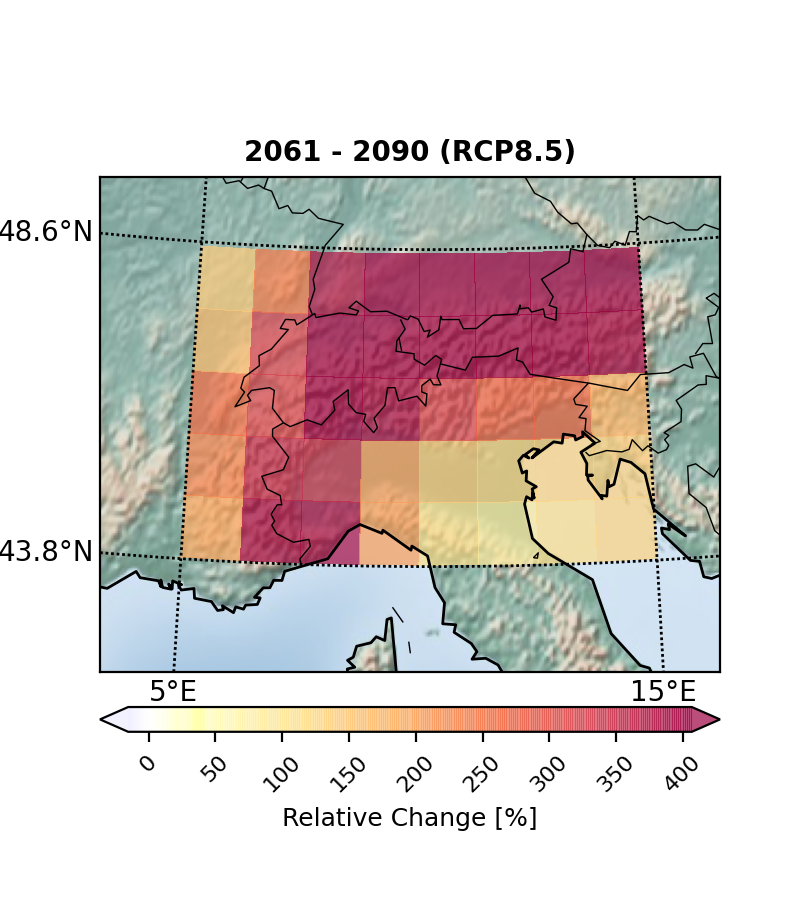
\includegraphics[trim=0 13 0 40, clip,width=.41\textwidth] {risultati/su_future_2061-2090_sub_rel}}
\end{center}
\end{frame}

%--------------------------------------------------

\begin{frame}
\frametitle{Cold Days}
\begin{center}

{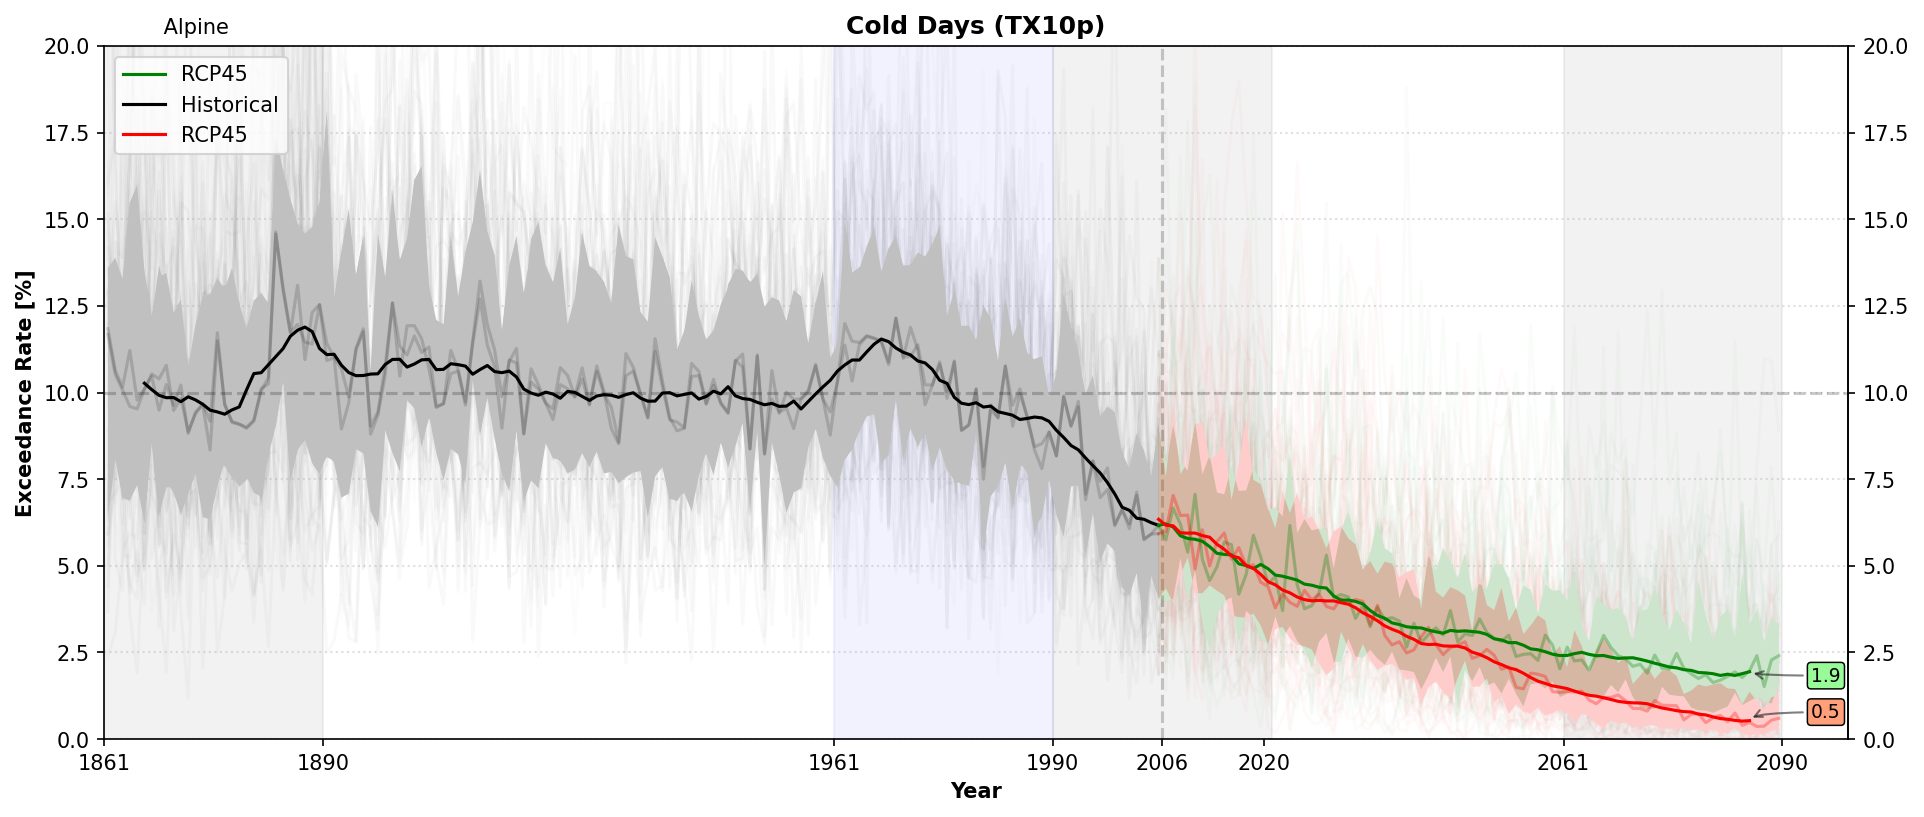
\includegraphics[width=0.8\textwidth]{risultati/tx10p_Alpine_Models_ts_lim_20}}
{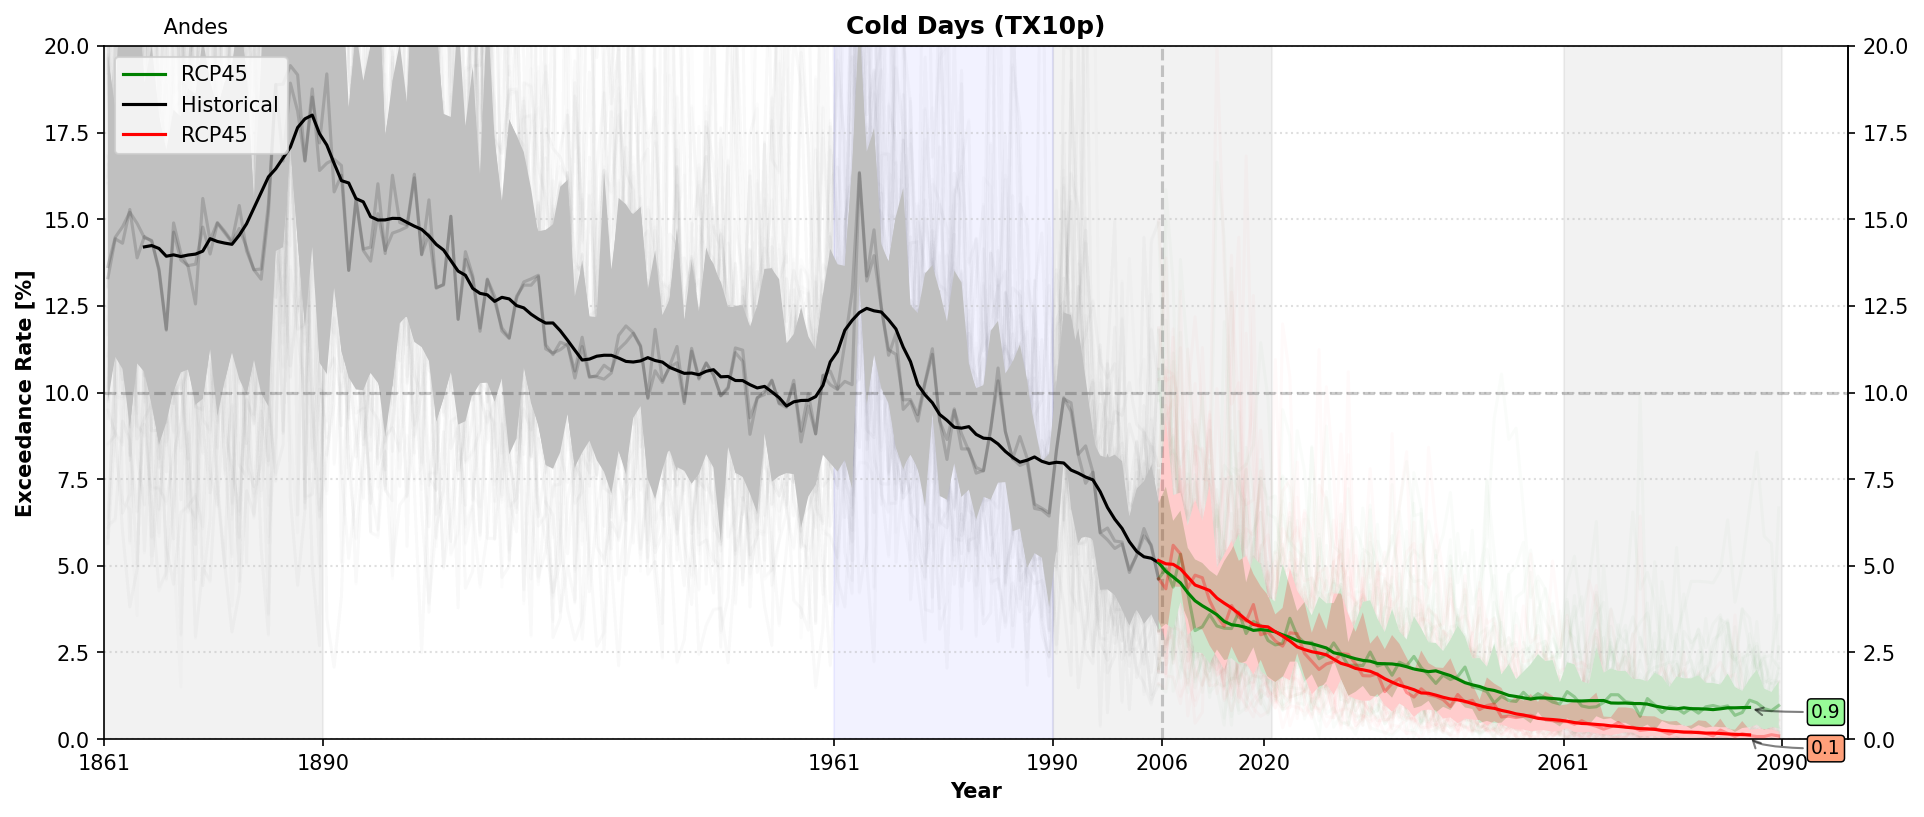
\includegraphics[width=0.8\textwidth]{risultati/tx10p_Andes_Models_ts_lim_20}}
\end{center}

{
  \scriptsize
  \begin{textblock}{1.8}(0.6,3)
     {\color{gray} Le Alpi}
  \end{textblock}
}


{
  \scriptsize
  \begin{textblock}{1.8}(0.6,9.5)
     {\color{gray} Le Ande}
  \end{textblock}
}

{ \tiny
  \begin{textblock}{3}(14,3)
     {\color{CadetBlue}  \texttt{10 \% : Rif}} \\
     {\color{ForestGreen}\texttt{1.9\%}} \\
     {\color{red}        \texttt{0.5\%}}
  \end{textblock}
}

{ \tiny
  \begin{textblock}{3}(14,9.5)
     {\color{CadetBlue}   \texttt{10 \% : Rif}} \\
     {\color{red}         \texttt{0.9\%}} \\
     {\color{ForestGreen} \texttt{0.1\%}}
  \end{textblock}
}

\end{frame}



%--------------------------------------------------

\begin{frame}
\frametitle{Precipitation extremes - R95p}
\begin{center}

{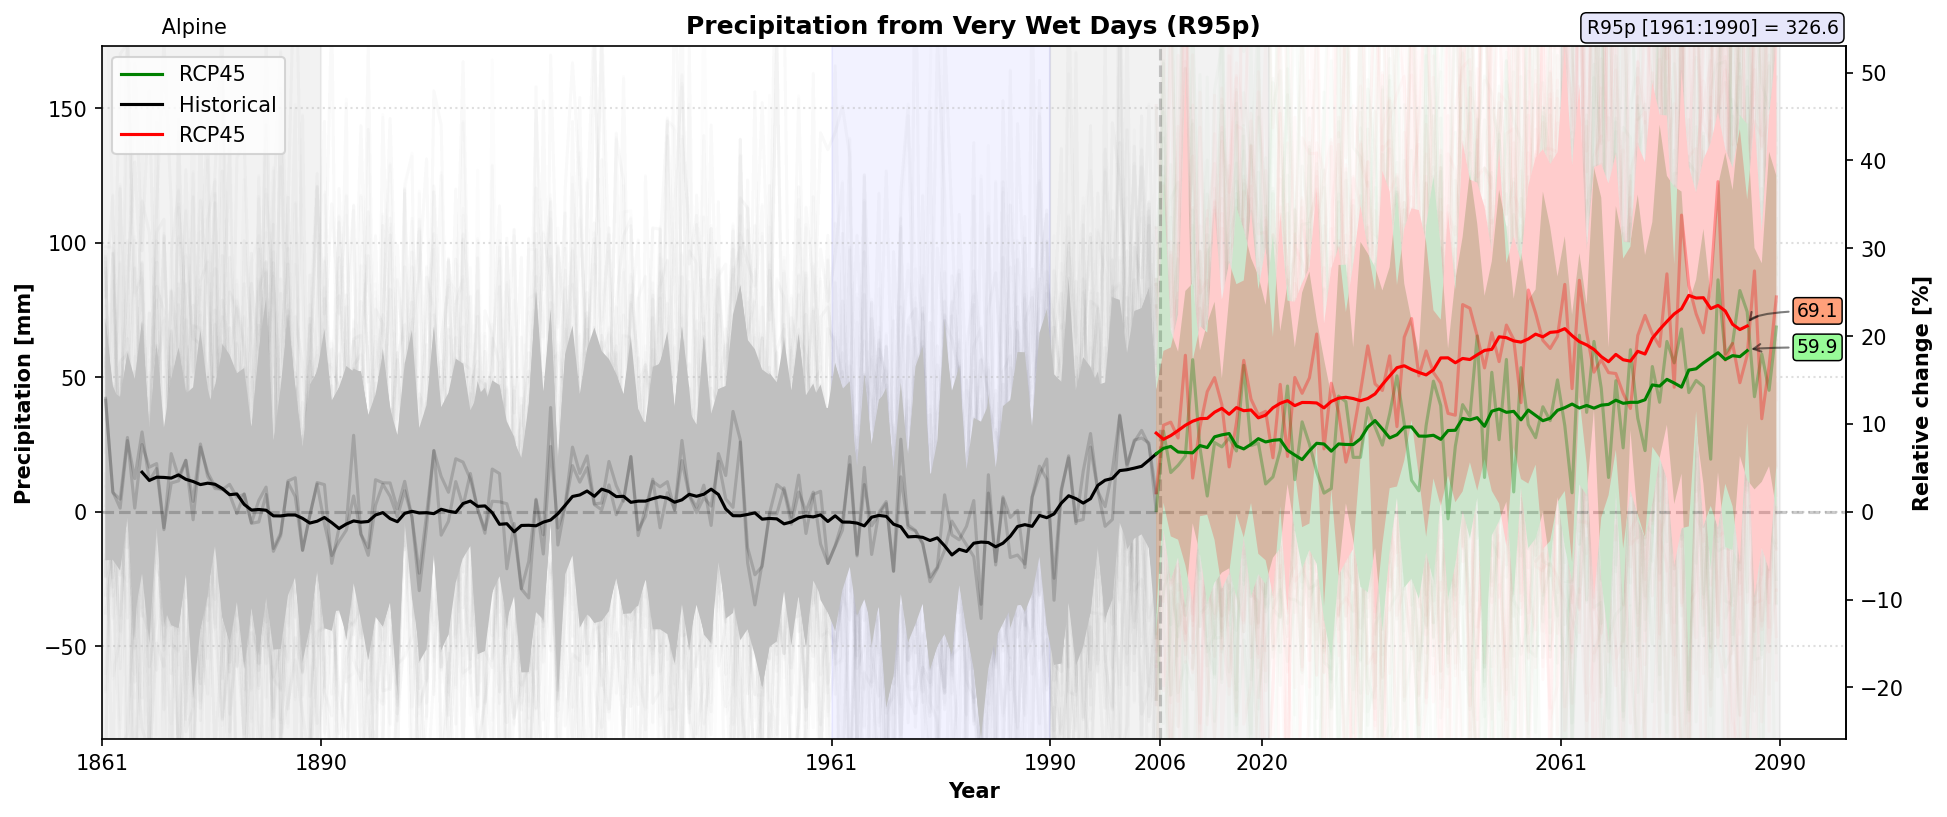
\includegraphics[width=0.8\textwidth]{risultati/r95p_Alpine_Models_ts}}
{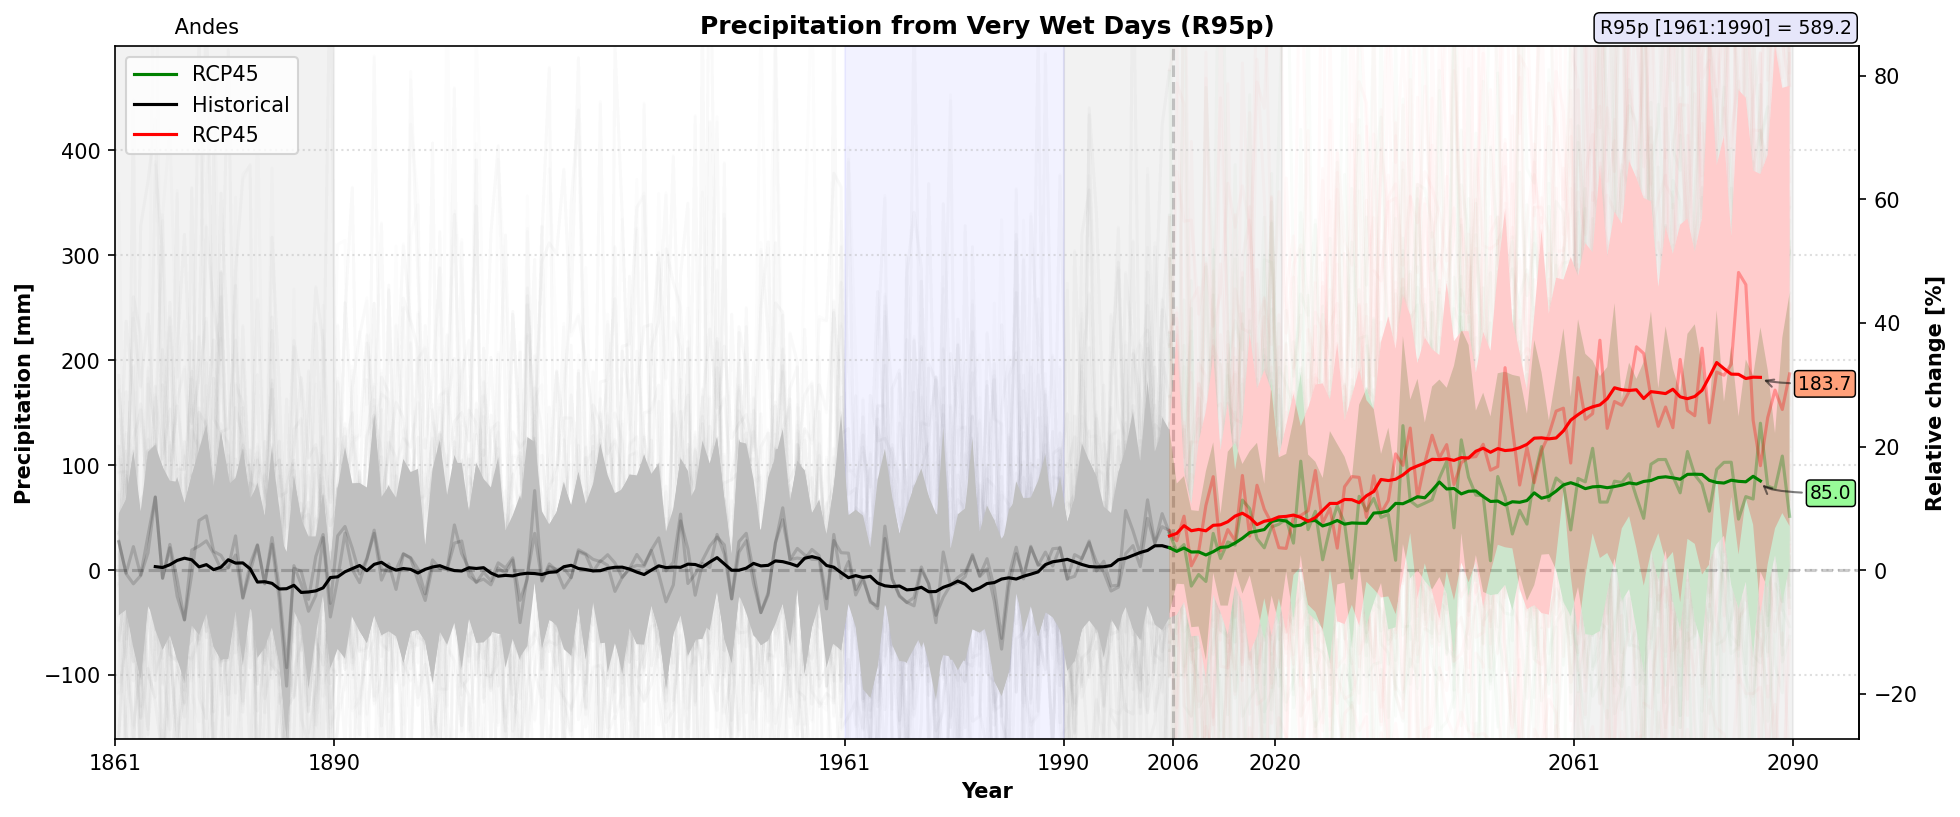
\includegraphics[width=0.8\textwidth]{risultati/r95p_Andes_Models_ts}}
\end{center}

{
  \scriptsize
  \begin{textblock}{1.8}(0.6,3)
     {\color{gray} Le Alpi}
  \end{textblock}
}


{
  \scriptsize
  \begin{textblock}{1.8}(0.6,9.5)
     {\color{gray} Le Ande}
  \end{textblock}
}

{ \tiny
  \begin{textblock}{3}(14,3)
     {\color{CadetBlue}   \texttt{326 mm : Rif}} \\
     {\color{red}         \texttt{ 69 mm : 21\% }}\\
     {\color{ForestGreen} \texttt{ 60 mm : 18\% }}
  \end{textblock}
}

{ \tiny
  \begin{textblock}{3}(14,9.5)
     {\color{CadetBlue}   \texttt{589 mm : Rif}} \\
     {\color{red}         \texttt{184 mm : 31\% }} \\
     {\color{ForestGreen} \texttt{ 85 mm : 14\%  }}
  \end{textblock}
}

\end{frame}

%--------------------------------------------------
\begin{frame}
\frametitle{Precipitation extremes - R95p}
\begin{center}

{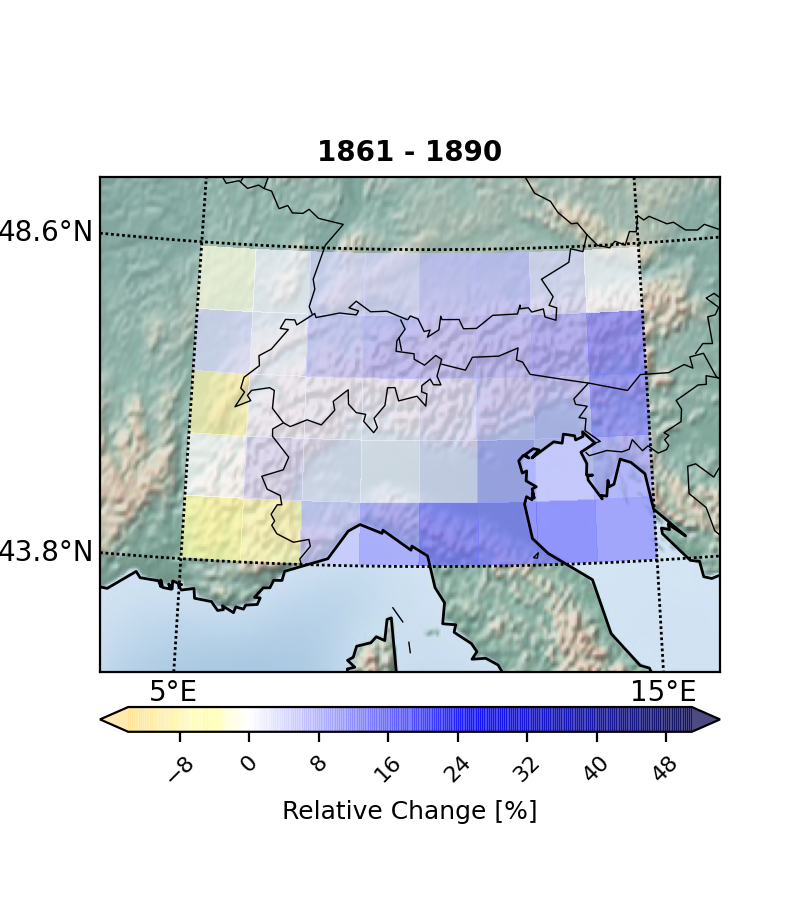
\includegraphics[trim=0 71 0 40, clip,width=.41\textwidth] {risultati/r95p_past_1861-1890_sub_rel}}
{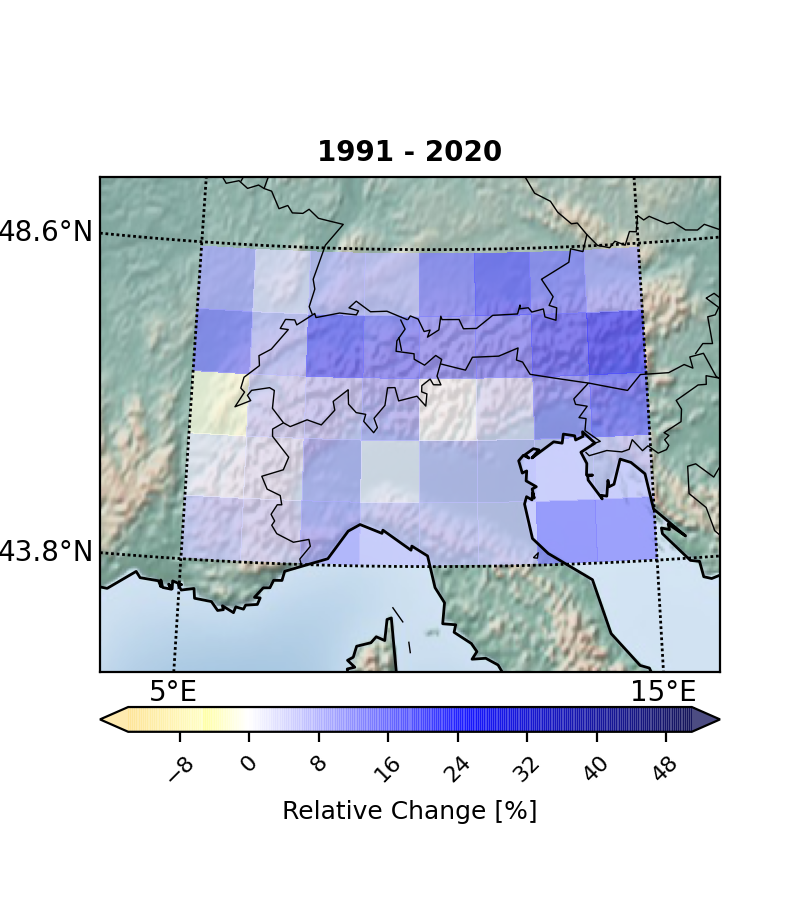
\includegraphics[trim=0 71 0 40, clip,width=.41\textwidth] {risultati/r95p_present_1991-2020_sub_rel}}
{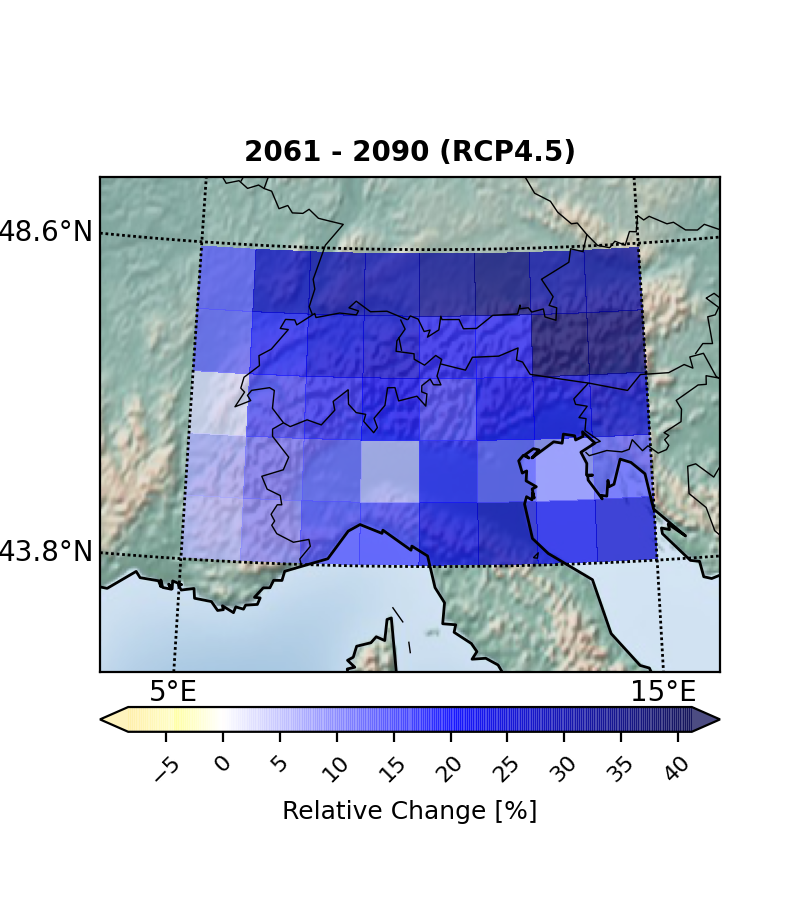
\includegraphics[trim=0 13 0 40, clip,width=.41\textwidth] {risultati/r95p_future_2061-2090_sub_rel_45}}
{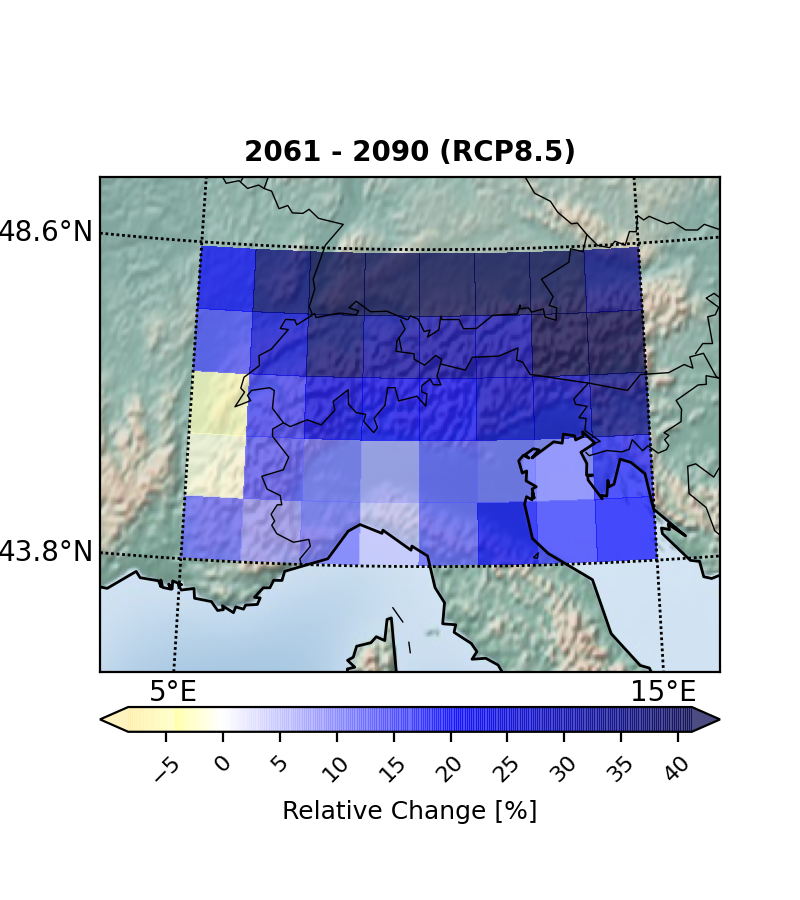
\includegraphics[trim=0 13 0 40, clip,width=.41\textwidth] {risultati/r95p_future_2061-2090_sub_rel}}
\end{center}
\end{frame}

%--------------------------------------------------

\begin{frame}
\frametitle{Precipitation extremes - PRCPTOT}
\begin{center}

{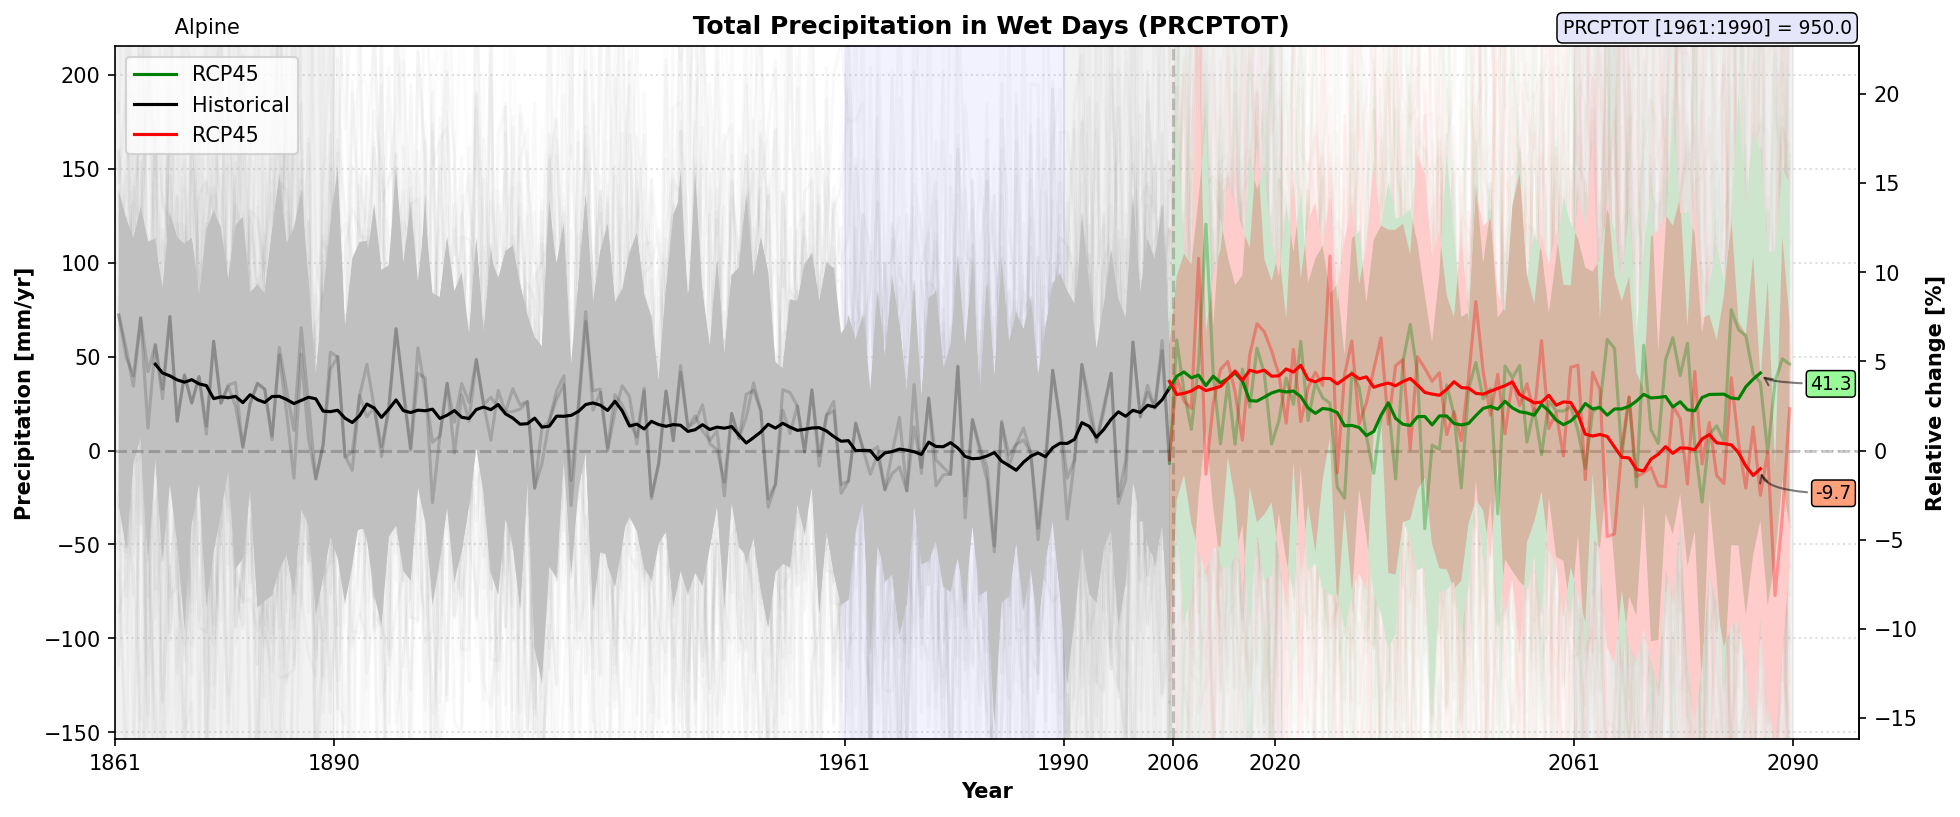
\includegraphics[width=0.8\textwidth]{risultati/prcptot_Alpine_Models_ts}}
{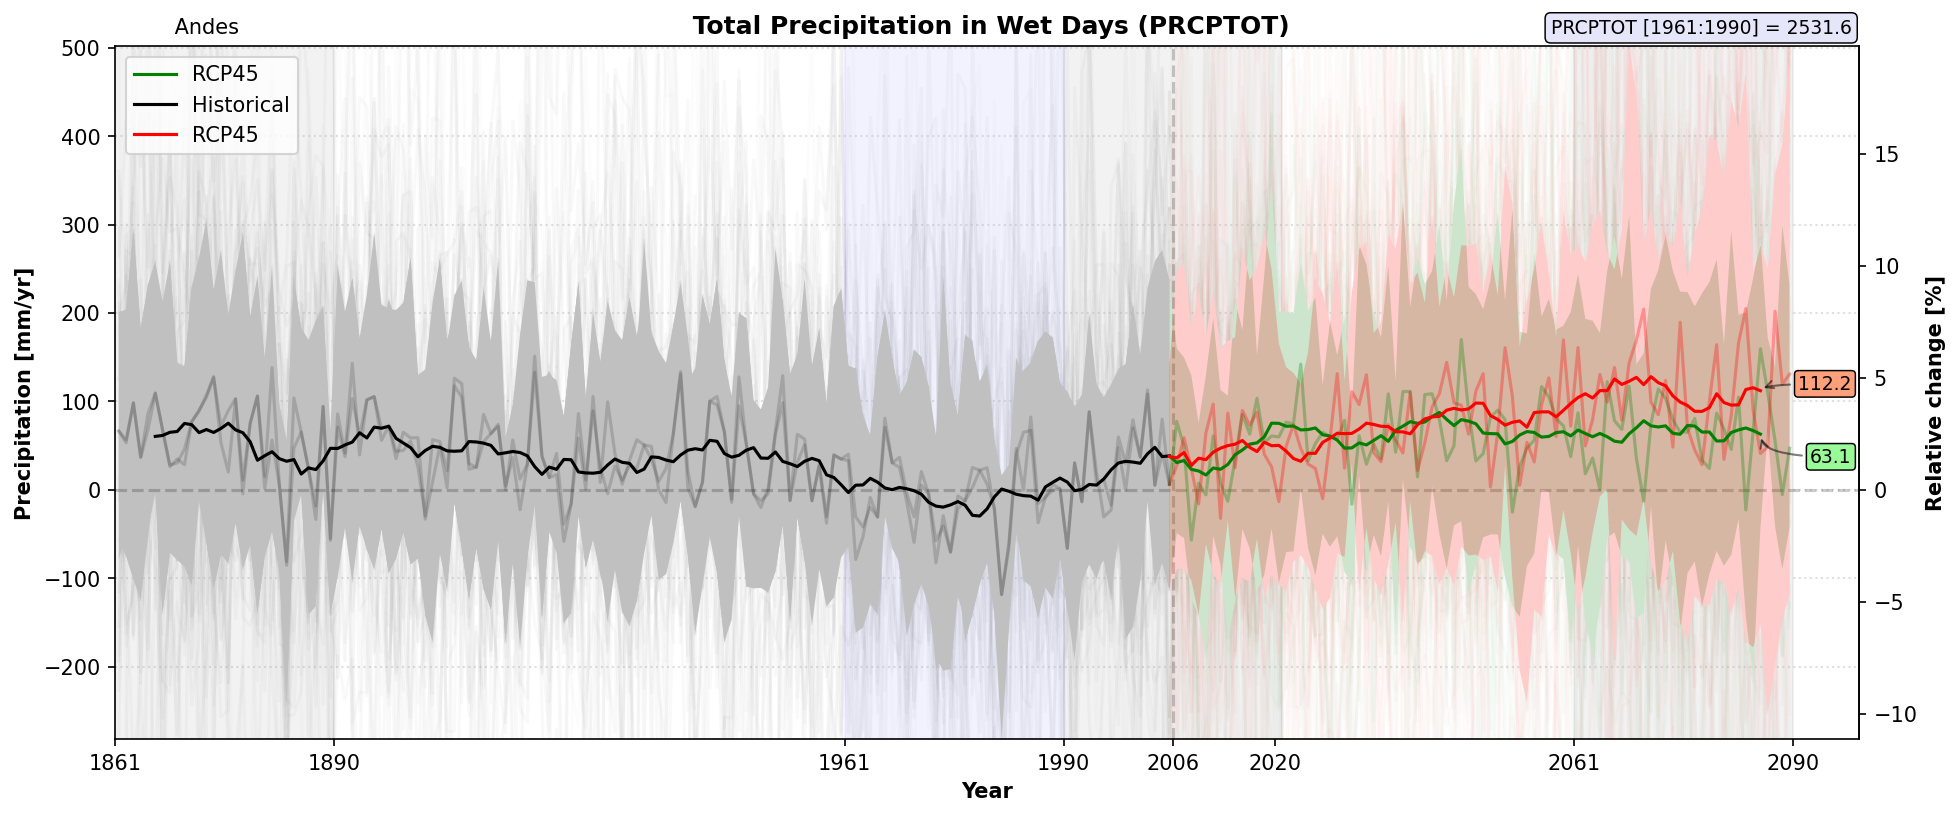
\includegraphics[width=0.8\textwidth]{risultati/prcptot_Andes_Models_ts}}
\end{center}

{
  \scriptsize
  \begin{textblock}{1.8}(0.6,3)
     {\color{gray} Le Alpi}
  \end{textblock}
}


{
  \scriptsize
  \begin{textblock}{1.8}(0.6,9.5)
     {\color{gray} Le Ande}
  \end{textblock}
}

{ \tiny
  \begin{textblock}{3}(13.8,3)
     {\color{CadetBlue}   \texttt{950 mm : Rif}} \\
     {\color{red}         \texttt{ 41 mm : 4.3\% }}\\
     {\color{ForestGreen} \texttt{-10 mm : \ -1\% }}
  \end{textblock}
}

{ \tiny
  \begin{textblock}{3}(13.7,9.5)
     {\color{CadetBlue}   \texttt{2531 mm : Rif}} \\
     {\color{red}         \texttt{ 112  mm : 4.4\% }} \\
     {\color{ForestGreen} \texttt{ \ 63  mm : 2.5\%  }}
  \end{textblock}
}

\end{frame}

%--------------------------------------------------
%\begin{frame}
%\frametitle{Precipitation extremes}
%\begin{center}
%
%{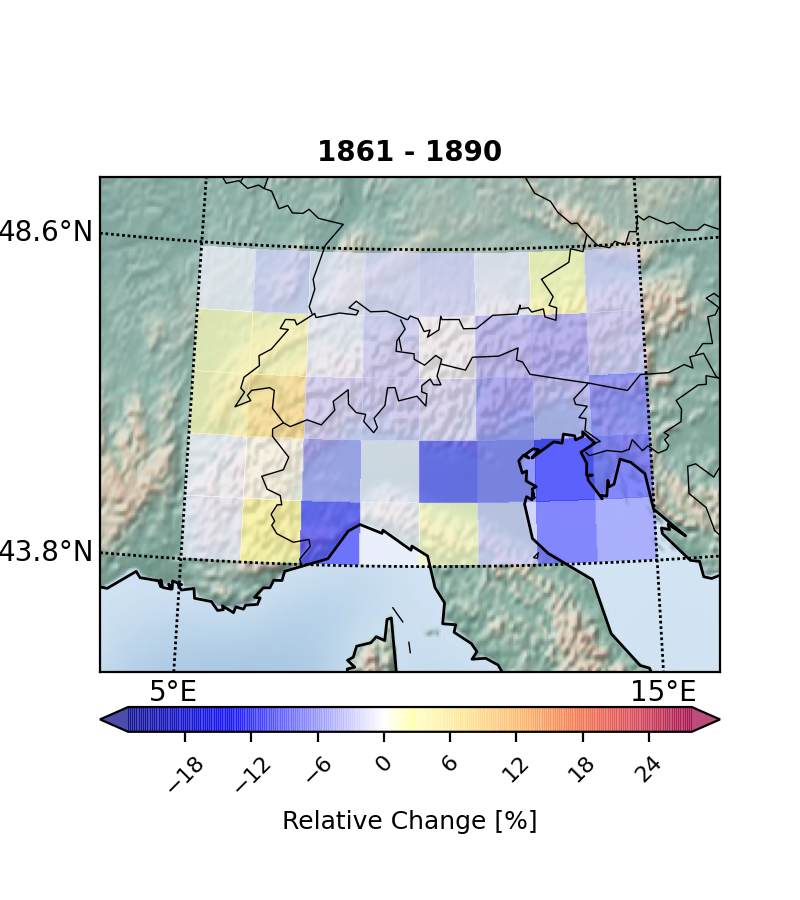
\includegraphics[trim=0 71 0 40, clip,width=.41\textwidth] {risultati/cdd_past_1861-1890_sub_rel}}
%{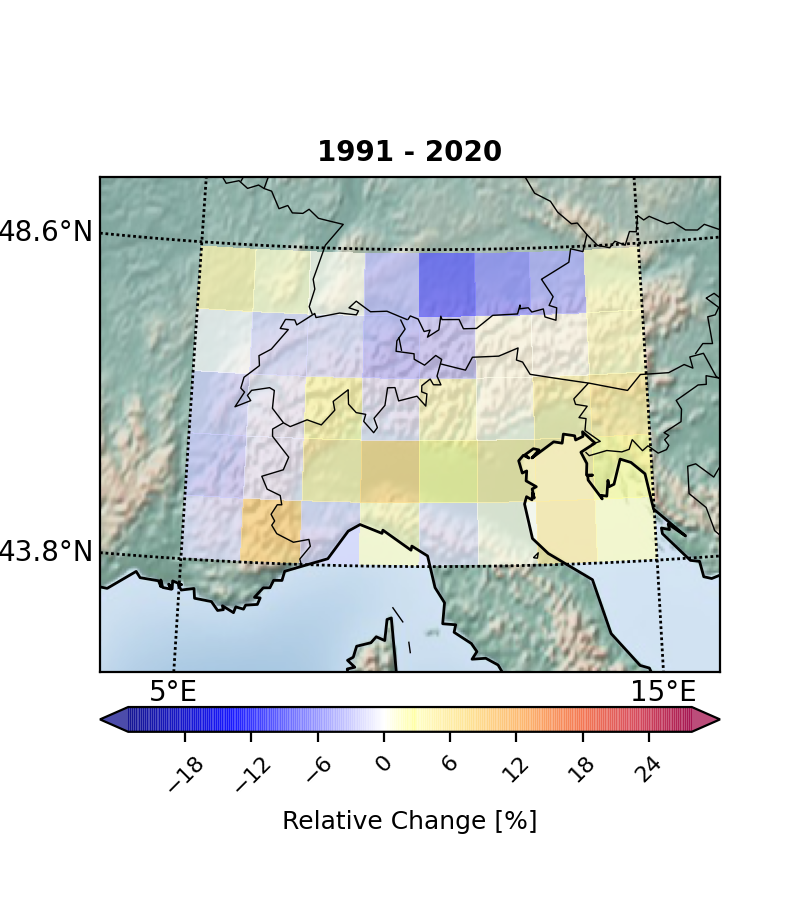
\includegraphics[trim=0 71 0 40, clip,width=.41\textwidth] {risultati/cdd_present_1991-2020_sub_rel}}
%{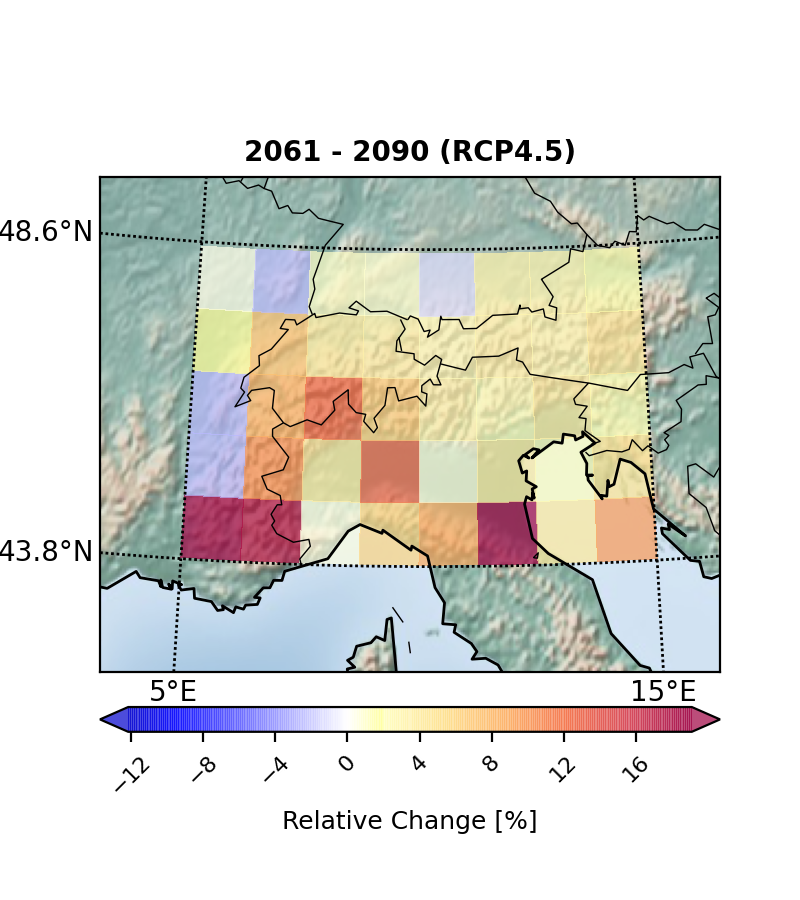
\includegraphics[trim=0 13 0 40, clip,width=.41\textwidth] {risultati/cdd_future_2061-2090_sub_rel45}}
%{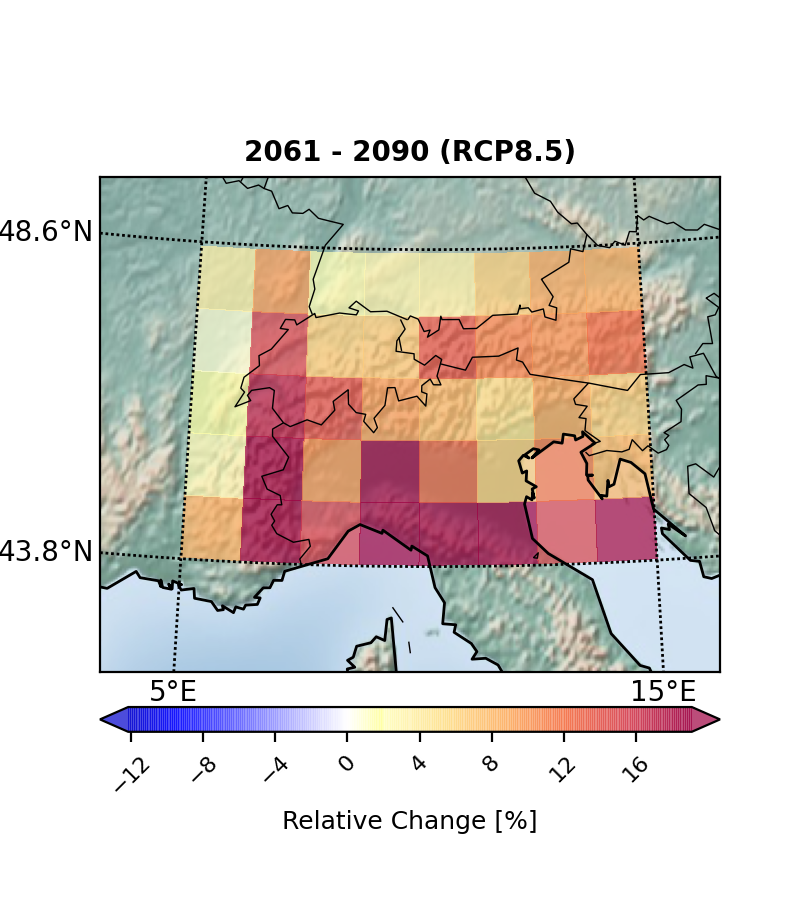
\includegraphics[trim=0 13 0 40, clip,width=.41\textwidth] {risultati/cdd_future_2061-2090_sub_rel}}
%\end{center}
%\end{frame}
